\documentclass[]{report}
\renewcommand\thesection{\arabic{section}}%for page numbering in arabics
\usepackage{graphicx,tabularx}%for figures and tables
\usepackage[utf8]{inputenc} %allows special characters such as ä, ö, ỳ
\usepackage[english]{babel}  %set the language to English
\usepackage[margin=1.5in]{geometry} %change page margins 
\usepackage{sectsty}%section headers
\allsectionsfont{\sffamily\large}
\subsectionfont{\sffamily\normalsize}
\linespread{1.2}% line distance
\usepackage{lipsum}% http://ctan.org/pkg/lipsum
\usepackage{caption}%use for captions on tables
%use this exact command. The style and bibliographystyle has to be authoryear (Havard). The sorting is nyt: name, year, title so that the bibliography is sorted alphabetically. firstinits=true shortens the names: Albert Einstein -> A. Einstein
\usepackage[backend=bibtex,style=authoryear,bibstyle=authoryear,sorting=nyt,firstinits=true]{biblatex}
\setlength\parindent{0pt}%include this so that your paragraphs don't indent automatically
\addbibresource{report.bib} %this attaches your bib-file, your bibliography (must be in the same folder)
\usepackage[compact]{titlesec}%include title formatting package

% Title Page
\title{Top Text}
\author{Tom Jacobs and James Boogaard}
\date{December 15th 2022 \\Module: SEAR \\Venlo, Limburg, Netherlands}


\begin{document}
	
	\maketitle
	
	\begin{abstract}
		This is the abstract.
		
		\pagenumbering{roman}
		
	\end{abstract}
	
	\tableofcontents
	\setcounter{page}{3}
	\listoffigures %UNCOMMENT IF YOU HAVE FIGURES
	%\listoftables %UNCOMMENT IF YOU HAVE TABLES
	\pagebreak
	
	\pagenumbering{arabic}	
	
	\section{Introduction}
During the year of 2022 there has been a massive increase in the popularity and use of text-to-image generators, an artificial intelligence technique that translates human text into a computer-generated image. You will likely have heard of at least one of these if you frequent the internet. This explosion in popularity has led to many different text-to-image applications being made, which on the one hand has given many more options to artists, (people who use a text-to-image generator to create and refine an image), but it has also made the landscape more difficult to navigate because of its abundance of choice. This paper makes an effort to try and alleviate this problem by picking four of the most used text-to-image generators and comparing them based on their accuracy and process so we can help people gain some perspective on which text-to-image generator is best for their needs.

A research paper was published on the nineteenth of February 2020 called: "A survey and taxonomy of adversarial neural networks for text-to-image synthesis" that makes use of surveys to compare models for text-to-image generations. This paper aimed to show which text-to-image technique yielded the most realistic results in a wide variety of categories. One issue with this paper was that is was written before the explosion of consumer text-to-image generators happened, which is why we will instead focus on modern consumer-grade generators which are available today. Another issue is that they don't allow average inexperienced artists to use their tools, instead their results are created by the researchers themselves. Because of this their results do not reflect what the average inexperienced artist can expect when using these text-to-image techniques. 

Our goal during the course of this research paper is to find out what the best text-to-image generator is, out of the four we chose, in the case of an artist who is not experienced in the world of text-to-image generation. Our hope is that artists that are new to text-to-image generation will be able to make an educated decision on which generator is best for them on the basis of this paper.

(? maybe instead focus on the tools inside the application.) Another question we take a look at is to find the best technique out of the four applications that we use and then analysing why that technique is so effective for artificial intelligence text-to-image generation. The techniques we will take a look at are latent diffusion, the V4 model, and VOGAN and CLIP.

The text-to-image generators we will be testing during the course of this paper are: Stable diffusion, Midjourney, DallE and Dream by Wombo. Stable diffusion was released in 2022 and makes use of the ai text-to-image synthesis technique known as latent diffusion. Midjourney which is currently in open beta and also makes use of latent diffusion to generate its images. DallE was released in January of 2021 and makes use of the V4 model to generate its images. Finally is dream by Wombo which was released in late 2021 and makes use of a combination of VOGAN and CLIP for text-to-image generation.

We expect the best text-to-image generator out of the four we chose to be stable diffusion. This is due to the fact that stable diffusion offers its users more tools and techniques like inpainting (allows you to regenerate a specific area of an image without regenerating the whole image), this allows the user more freedom to fine-tune their result. Given enough time this will yield a more accurate result. This however only applies for artists who are already experienced, because it can take quite some practice to get used to all the tools that are available in stable diffusion. We expect inexperienced artists to struggle finding the right settings because of the amount of freedom they get. In the case of a completely inexperienced artist, they might find Dall-E easier to use because it can create photorealistic results without having to fine tune any settings apart from the prompt.
	

	
	\section{Methods}
	
	Our goal during the course of this research paper is to find out what the best text to image generator is, out of the four we chose, for artists who are experienced as well as artists who are not experienced in AI art generation.
	
	(? Instead look at amount of tools available) A secondary research question that we take a look at in this paper is to find out the strengths of the different ai text to image generation techniques used in the applications we have chosen.
	
	This paper is used as an attempt to prove that stable diffusion is the best application out of the four, we chose. Our x value is the array of different applications that we use and the y value is the result of that (the distance) for each iteration on the road to trying to recreate an image using these applications. The intervening variable in this case would be the amount of experience using these applications.
	
	We have chosen an image that we find sufficiently covers all the challenging parts of recreating an image using ai art generation such as reflections and complex composition. We then use each of the four artificial intelligence applications to try and recreate that image within a given time frame (15 minutes). After each iteration we take the generated image (iteration) and add it to a list of the iterations that we created while recreating that image for that specific application(each application will thus have their own history of the process of the participants tying to recreate the image). With those sets of data, we then plug the images (each iteration) into an AI application that can give you a numerical value for how close one image is to another and see how close each iteration is to the image we are trying to recreate. this then gives us insight into how fast the application is (how efficient its technique is) and how many iterations you have to do to achieve a certain result. Once the data is gathered, we can create a graph to compare the applications more easily. The people that carried out this experiment also consisted of one novice and one experienced individual. This is to see which is the best application for each group of people and thus, the results will be conveyed on two separate graphs(one graph for each group of people). In terms of our secondary research question this method also gives us insight if we are aware of the techniques each of the ai generation applications use, we can notice if there is a pattern of success or failure with each and thus are able to compare them and see which one is the best.
	
	In order to compare the image generation applications effectively we observe a multitude of factors that will indicate the strengths and weaknesses of that application. These fators are: The amount of iterations each participant can generate while trying to create the image within the 15 minute time limit, how close each iteration is to the image we are trying to replicate using the ai image comparing program's unit of measurement (the unit is called distance. The closer to zero the distance is, the closer the images are together. zero means that the two images that are being compared are exactly the same), how easily we were able to access the application and its functionality, how much functionality each application offers and their effects on the final results of our experiment.
	
	
	We have chosen an image that we find sufficiently covers all the hard parts of recreating an image using ai art generation such as reflections and complex composition. We then use each of the four artificial intelligence applications to try and recreate that image within a given time frame (15 minutes). After each iteration we take that image and compile it into a list of the iterations for the process of recreating that image for that specific application. With those sets of data, we then run the images (each iteration) through an AI application developed by DeepAI that can give you a numerical value (distance) based on how close one image is to another, the lower the distance the closer the image. This way we can see how close each iteration is to the image we are trying to recreate.
	
	Once the data is gathered, we can create a graph to compare the applications more easily. The people that carried out this experiment also consisted of one novice and one experienced individual. This is to see which is the best application for each group of people and thus, the results will be conveyed on two separate graphs.
	
	In terms of our secondary research question this method also gives us insight if we are aware of the techniques each of them use we can notice if there is a pattern of success or failure with each.
	
	
	
	\section{Results}

	\newpage
    \begin{figure}
    	\centering
    	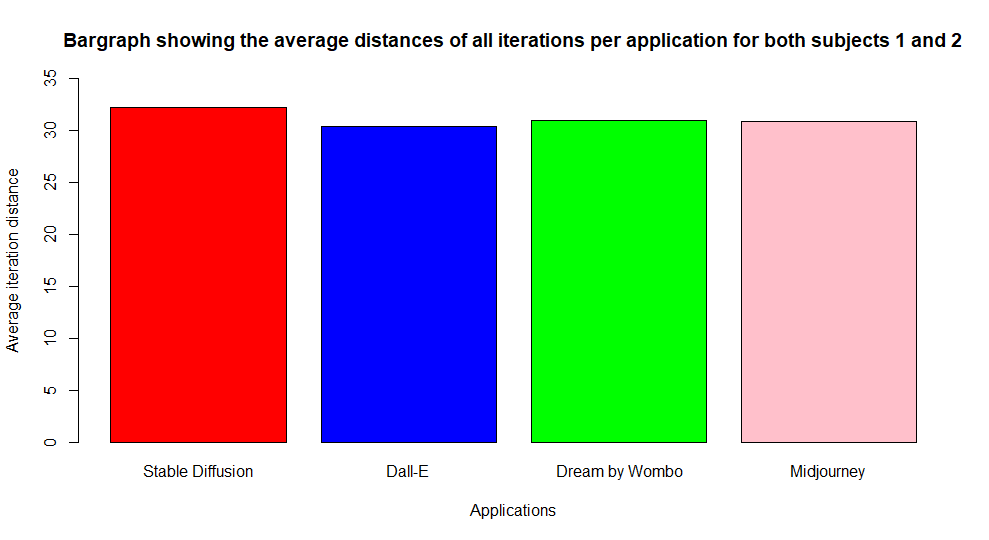
\includegraphics[width=1\linewidth]{Bargraph}
    	\caption{}
    	\label{fig:bargraph}
    \end{figure}
    
	\begin{figure}
		\centering
		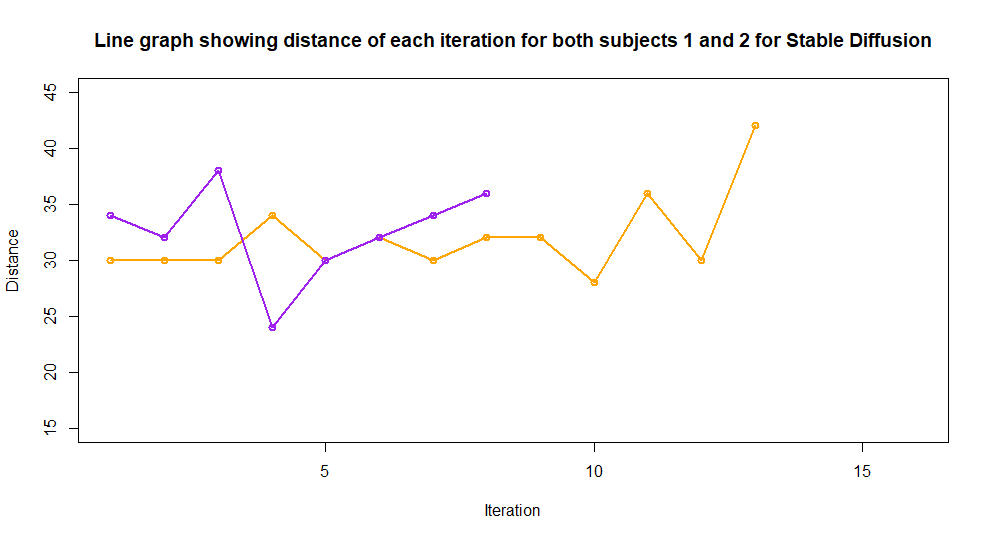
\includegraphics[width=1\linewidth]{LineGraphStableDiff}
		\caption{}
		\label{fig:linegraphstablediff}
	\end{figure}

	\begin{figure}
		\centering
		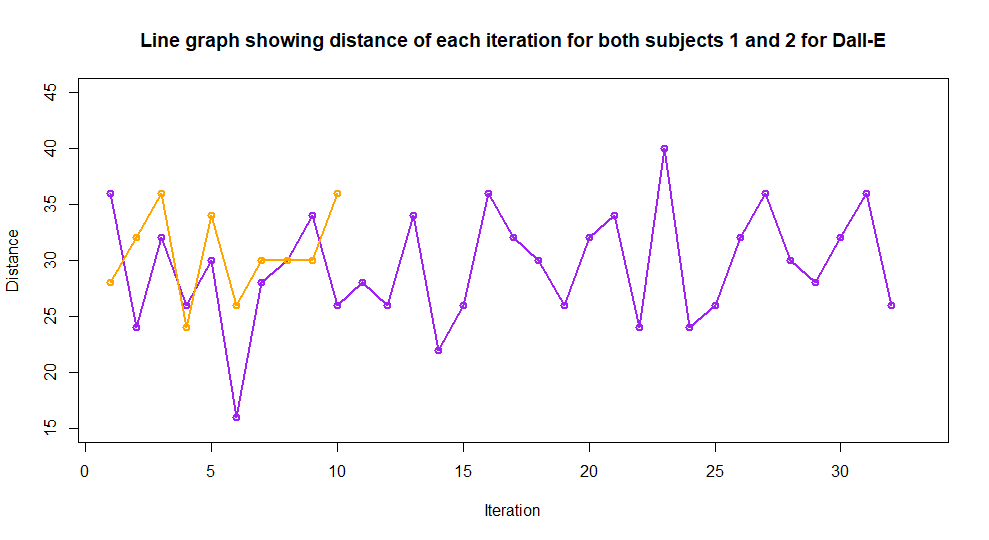
\includegraphics[width=1\linewidth]{LineGraphDall-E}
		\caption{}
		\label{fig:linegraphdall-e}
	\end{figure}
	
	
	\begin{figure}
		\centering
		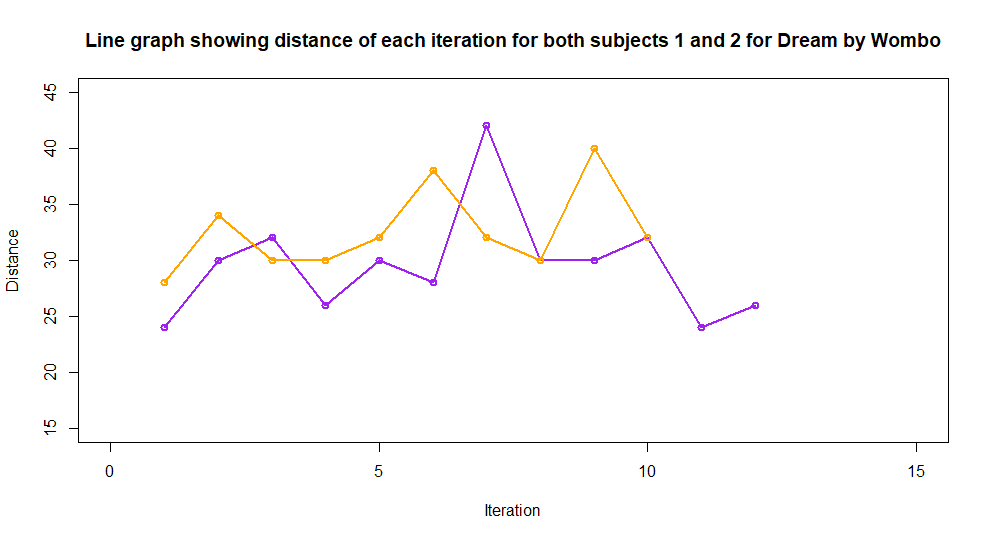
\includegraphics[width=1\linewidth]{LineGraphDBW}
		\caption{}
		\label{fig:linegraphdbw}
	\end{figure}
	
	
	\begin{figure}
		\centering
		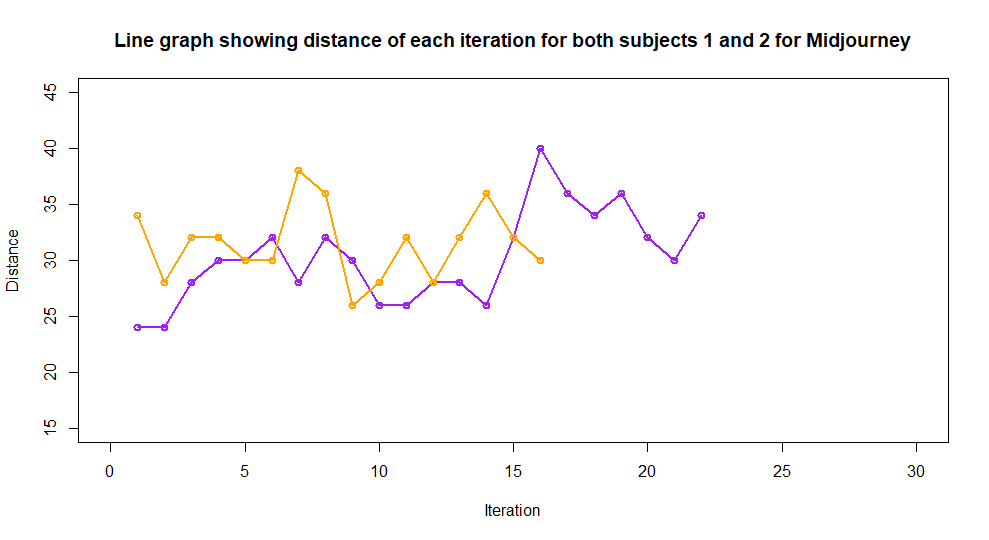
\includegraphics[width=1\linewidth]{LineGraphMidJ}
		\caption{}
		\label{fig:linegraphmidj}
	\end{figure}
	
	\begin{figure}
		\centering
		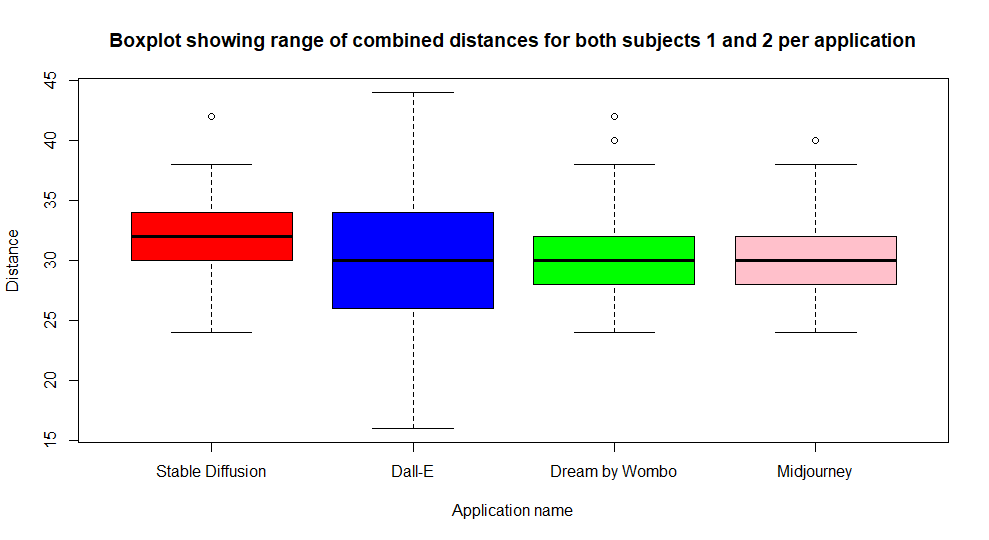
\includegraphics[width=1\linewidth]{boxplotWithAllData}
		\caption{}
		\label{fig:boxplotwithalldata}
	\end{figure}
	
	\section{Discussion}
	
\end{document}


\printbibliography[title=References]

\end{document}          
       
